\documentclass[12pt]{article}
\usepackage{amsmath,amssymb,amsthm}
\usepackage[margin=1in]{geometry}
\usepackage{graphicx,enumerate,fancyhdr,subfig,tikz,comment}
\usepackage[inline]{enumitem}
\usepackage[labelfont=bf]{caption}

\pagestyle{fancy}
\fancyhf{}
\chead{PROBLEM SET 1}
\rhead{Elliot Ahn}
\rfoot{\thepage}
\lhead{CS155}

\setlength{\headheight}{15pt}
\renewcommand{\footrulewidth}{0.5pt}

\newcommand{\E}{\mathbb E}
\newcommand{\Eout}{E_{\text{out}}}
\newcommand{\x}{\mathbf x}
\newcommand{\w}{\mathbf w}

\begin{document}

\begin{enumerate}[leftmargin=*]
\item
\begin{enumerate}[label = \Alph*.]
\item A hypothesis set is a set of possible models to approximate the target function.
\item Given input space $\mathcal X$, the hypothesis set of a linear model is a function of the form
\[ f(x) = w^T x + b \qquad \text{for } x \in \mathcal X\]
For classification, we would use
\[ f(x) = \text{sign}(w^T x + b) \]
\item Overfitting occurs when we choose a model of a sufficiently high complexity that reduces the in-sample error but increases the out-of-sample or test error.
\item The two ways to prevent overfitting is to have more data points or to use a regularization term, or use a simpler model. Regularization tends to penalize the higher-order (more complex) terms to favor the simpler models.
\item Training data is used to determine the parameter values of a model. Testing data is used to evaluate the performance of the model. If you change your information based on the test data, then you're effectively using test data as your training data, and your test data does not accurately reflect our-of-sample performance.
\item We assume that our data is identically and independently sampled from the same distribution.
\item The input space $\mathcal X$ could be the email address, the contents of the email using bagging of words, the title of the email (again using bagging of words). $Y$ would be a binary classification of `yes'-`no' for spam or not spam.
\item The $k$-fold CV procedure is to split the data into $k$ partitions. Then you train $k - 1$ of the partitions and test on the one partition to get a test error on the $i$th partition $E_i$. You run through this so that every partition eventually becomes a test partition and the cross-validation error is
\[ E_{CV} = \frac{1}{N} \sum_{i = 1}^N E_i. \]
\end{enumerate}
\item
\begin{enumerate}[label = \Alph*.]
\item 
\begin{align*}
\E_S [\Eout (f_S)] &= \E_S \left[ \E_x \left[ (f_S(x) - y(x))^2 \right] \right] \\
&= \E_S \left[ E_x \left[ (f_S(x) - F(x) + F(x) - y(x))^2 \right] \right] \\
&= \E_{S, x} \big[ \left( f_S(x) - F(x) \right)^2 + \left( F(x) - y(x) \right)^2 \\
& \qquad + f_S(x) F(x) - F(x)^2 - f_S(x) y(x) + F(x) y(x) \big] \\
&= \E_x \left[ \text{Bias}(x) + \text{Var}(x) \right]
\end{align*}
where the cross terms in the last step vanish to zero.
\item The learning curves are shown in figure \ref{fig1}.
\begin{figure}[h!]
\centering
\subfloat[$d = 1$]{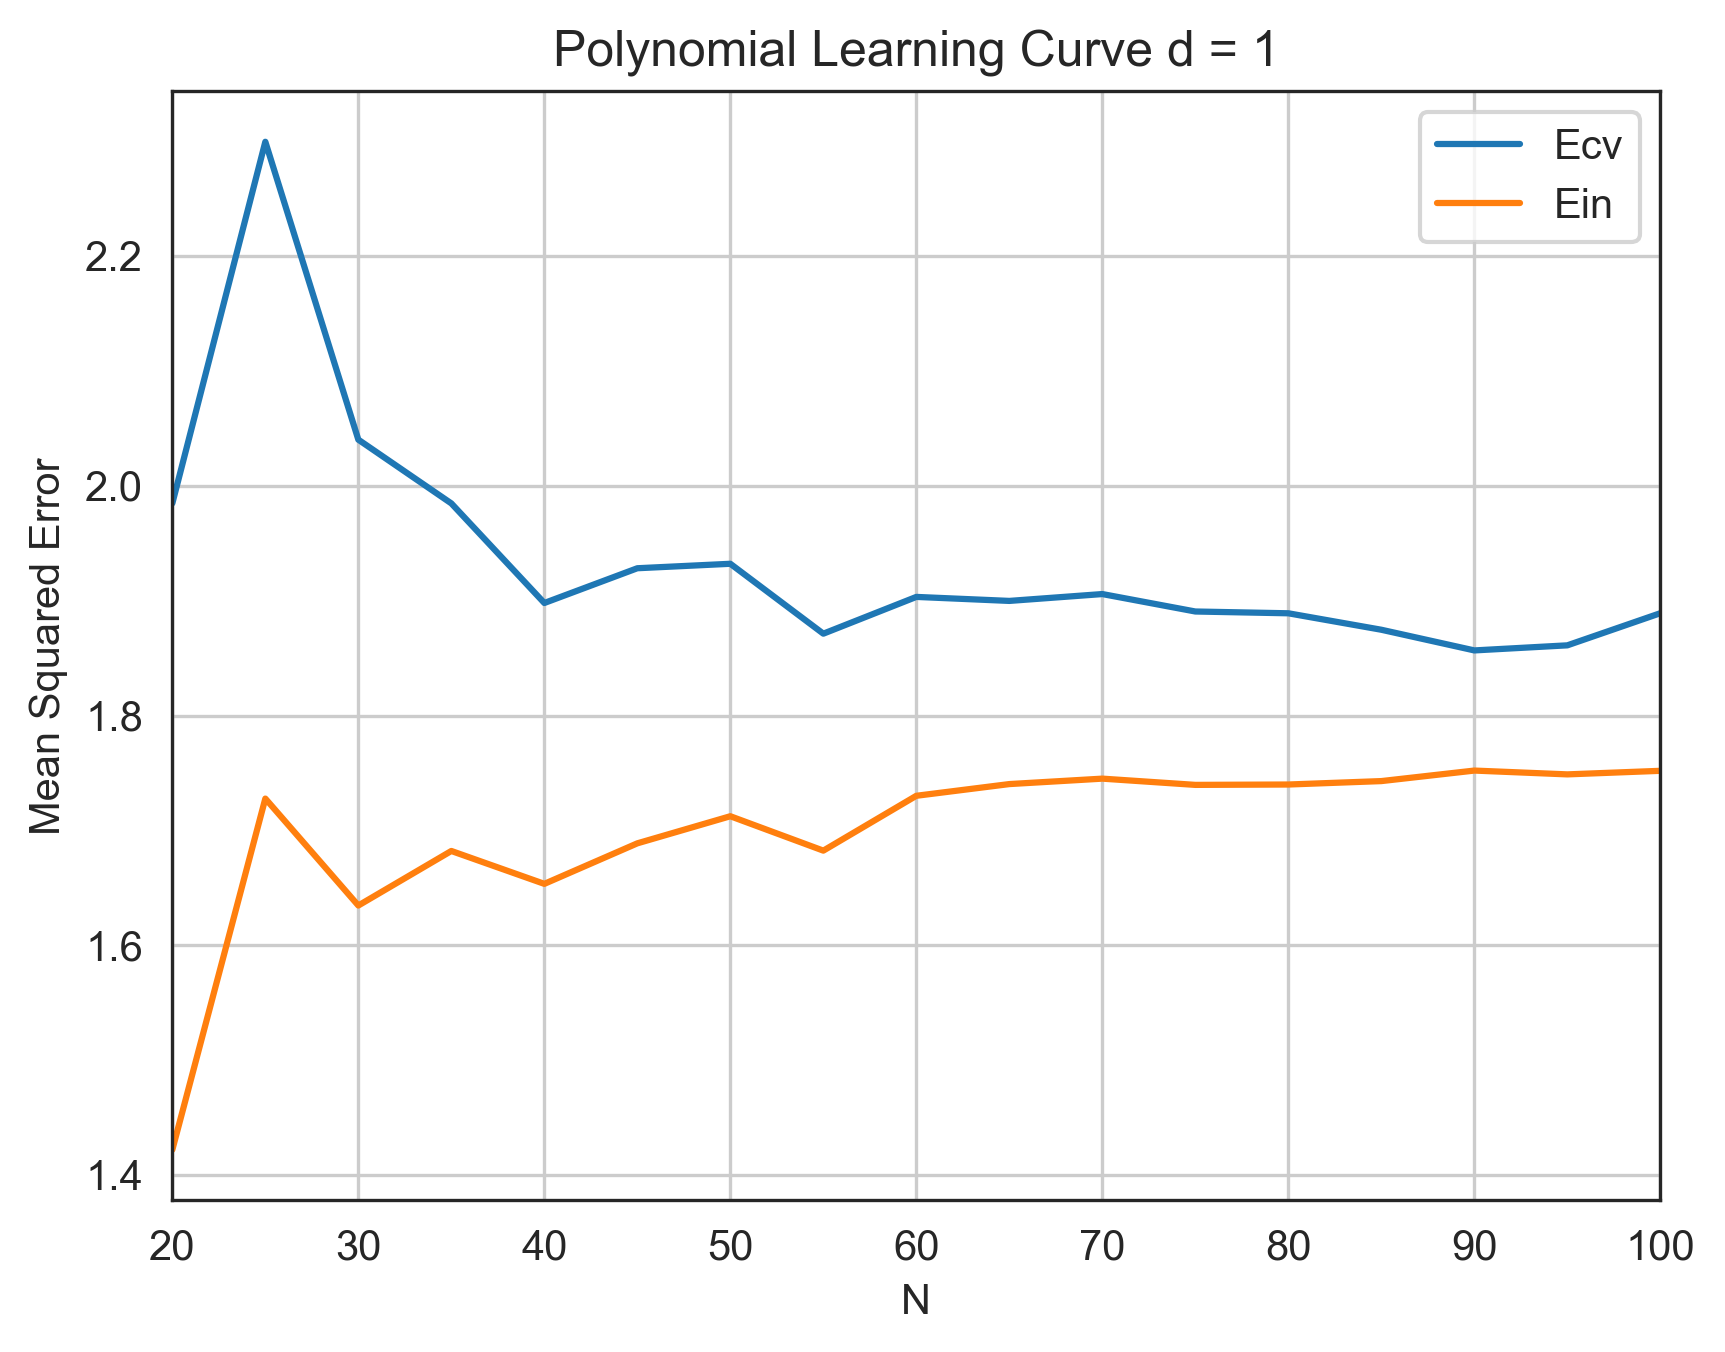
\includegraphics[scale=0.5]{figures/learncurve1.png}}
\subfloat[$d = 2$]{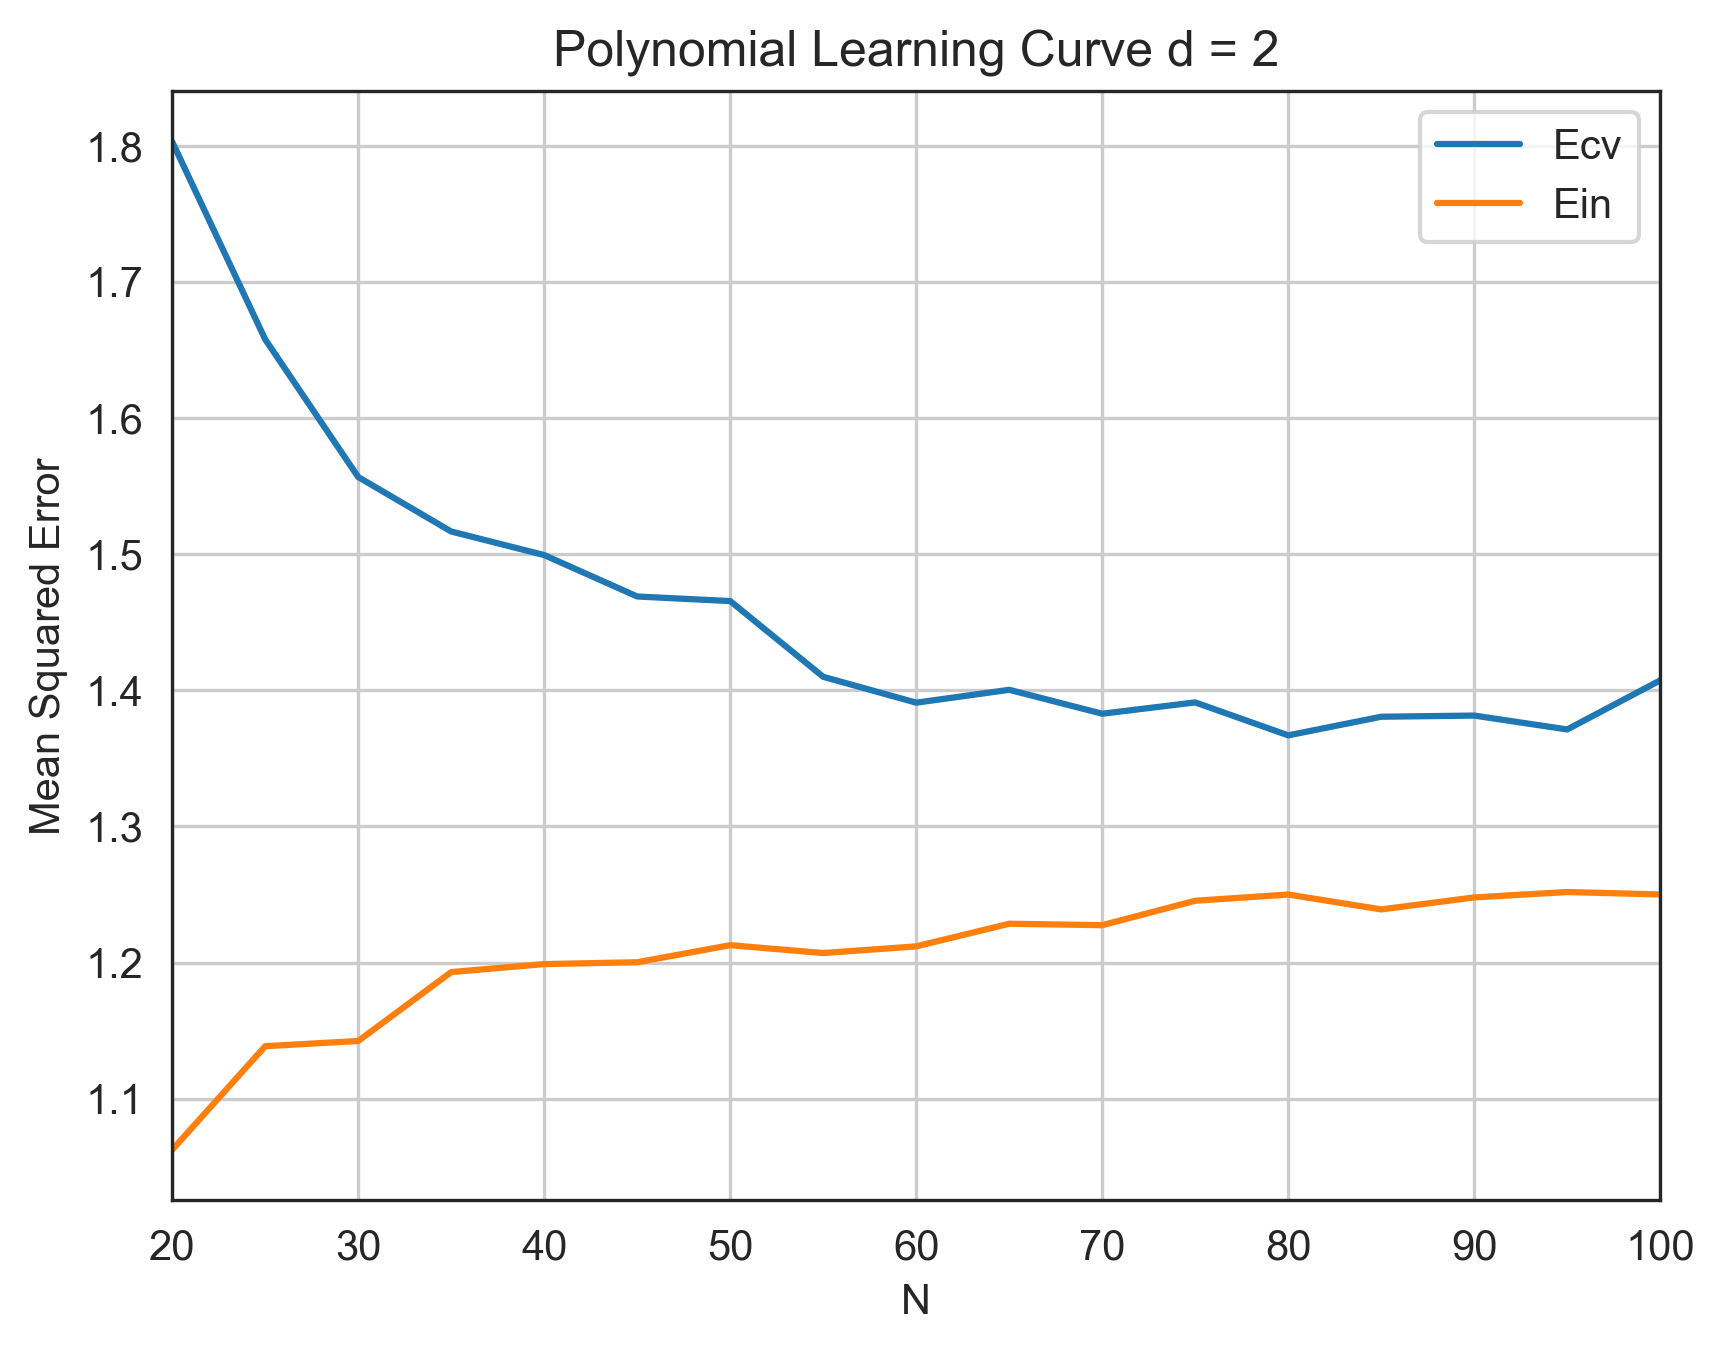
\includegraphics[scale=0.5]{figures/learncurve2.png}}
\hspace{0mm}
\subfloat[$d = 6$]{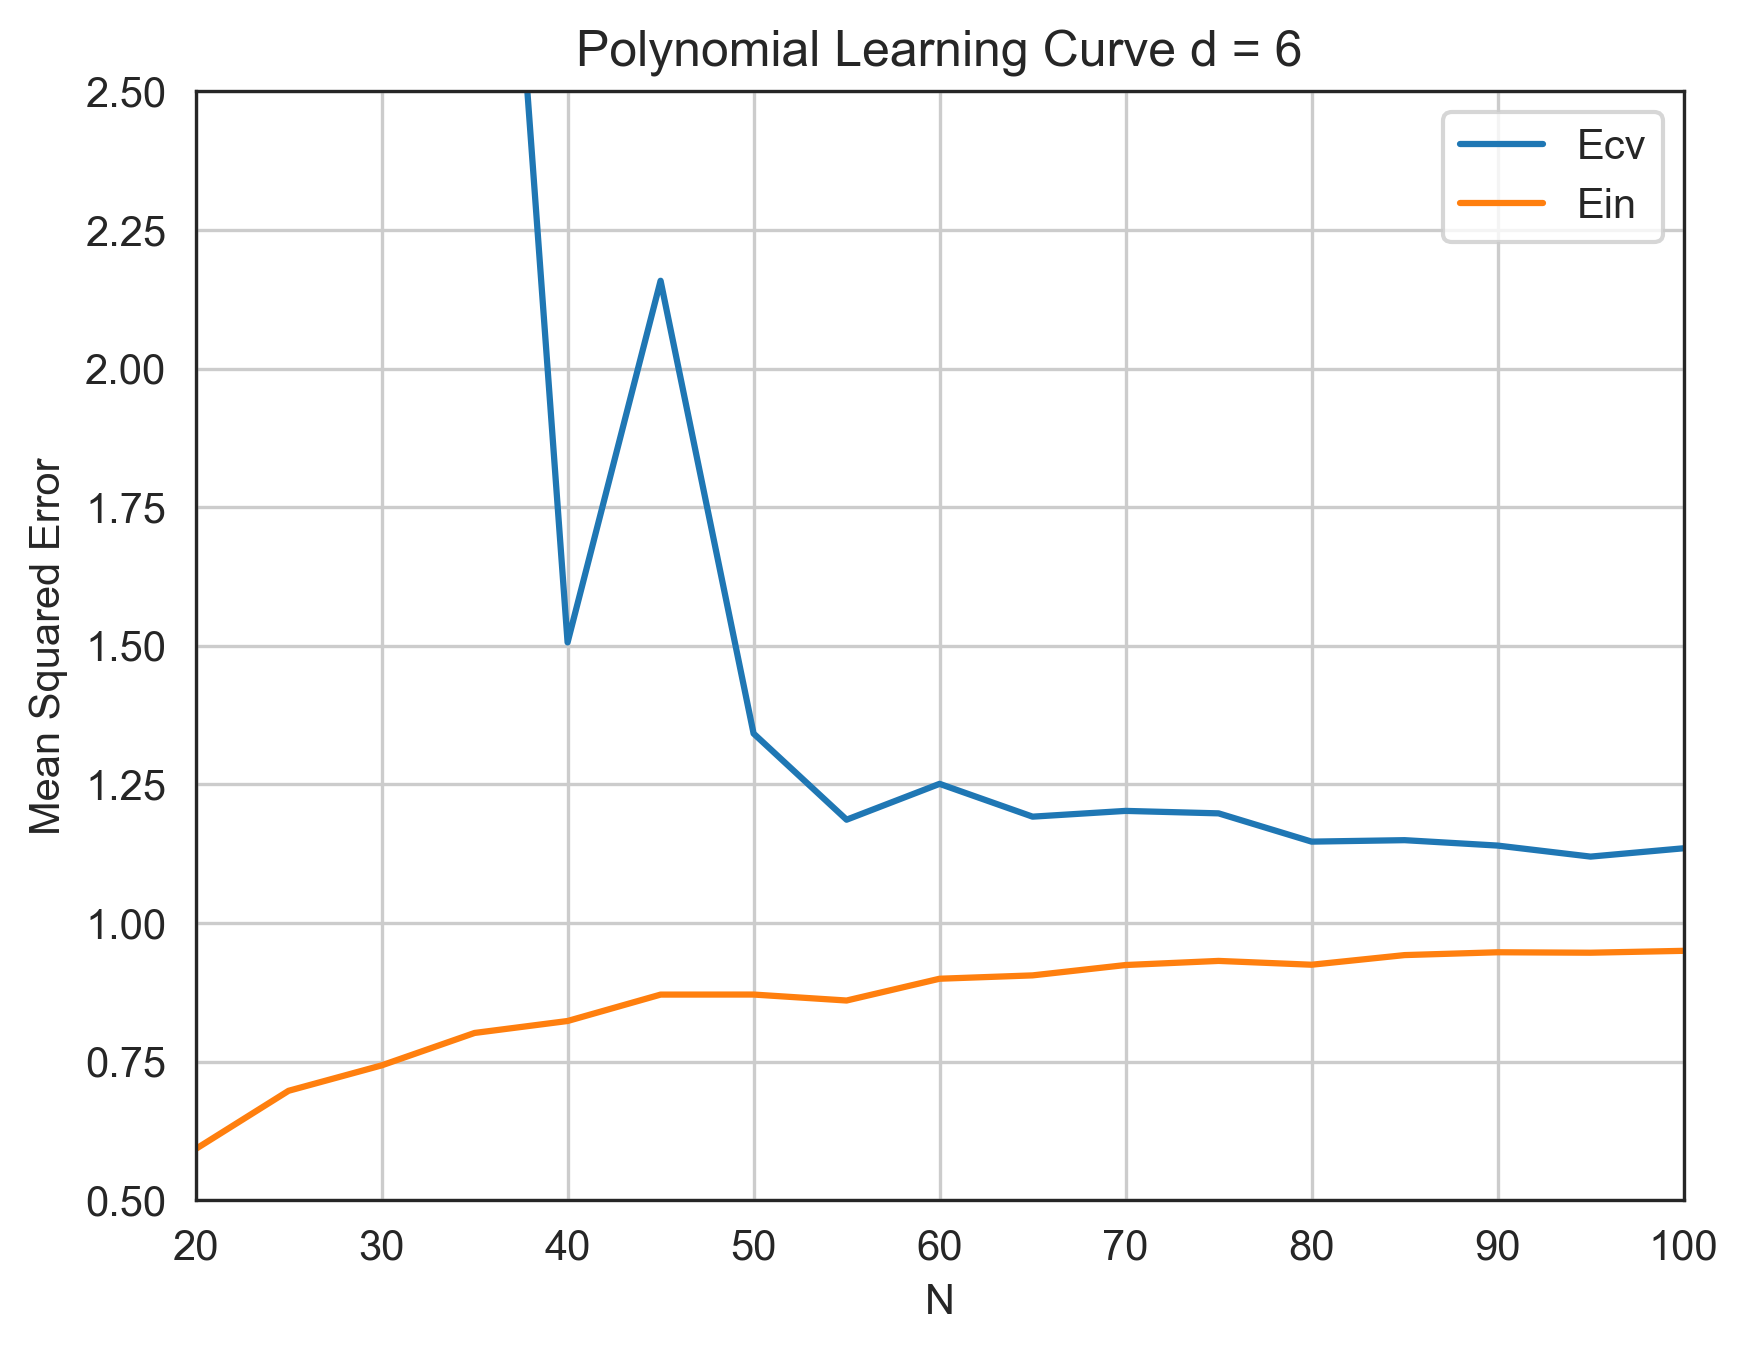
\includegraphics[scale=0.5]{figures/learncurve6.png}}
\subfloat[$d = 12$]{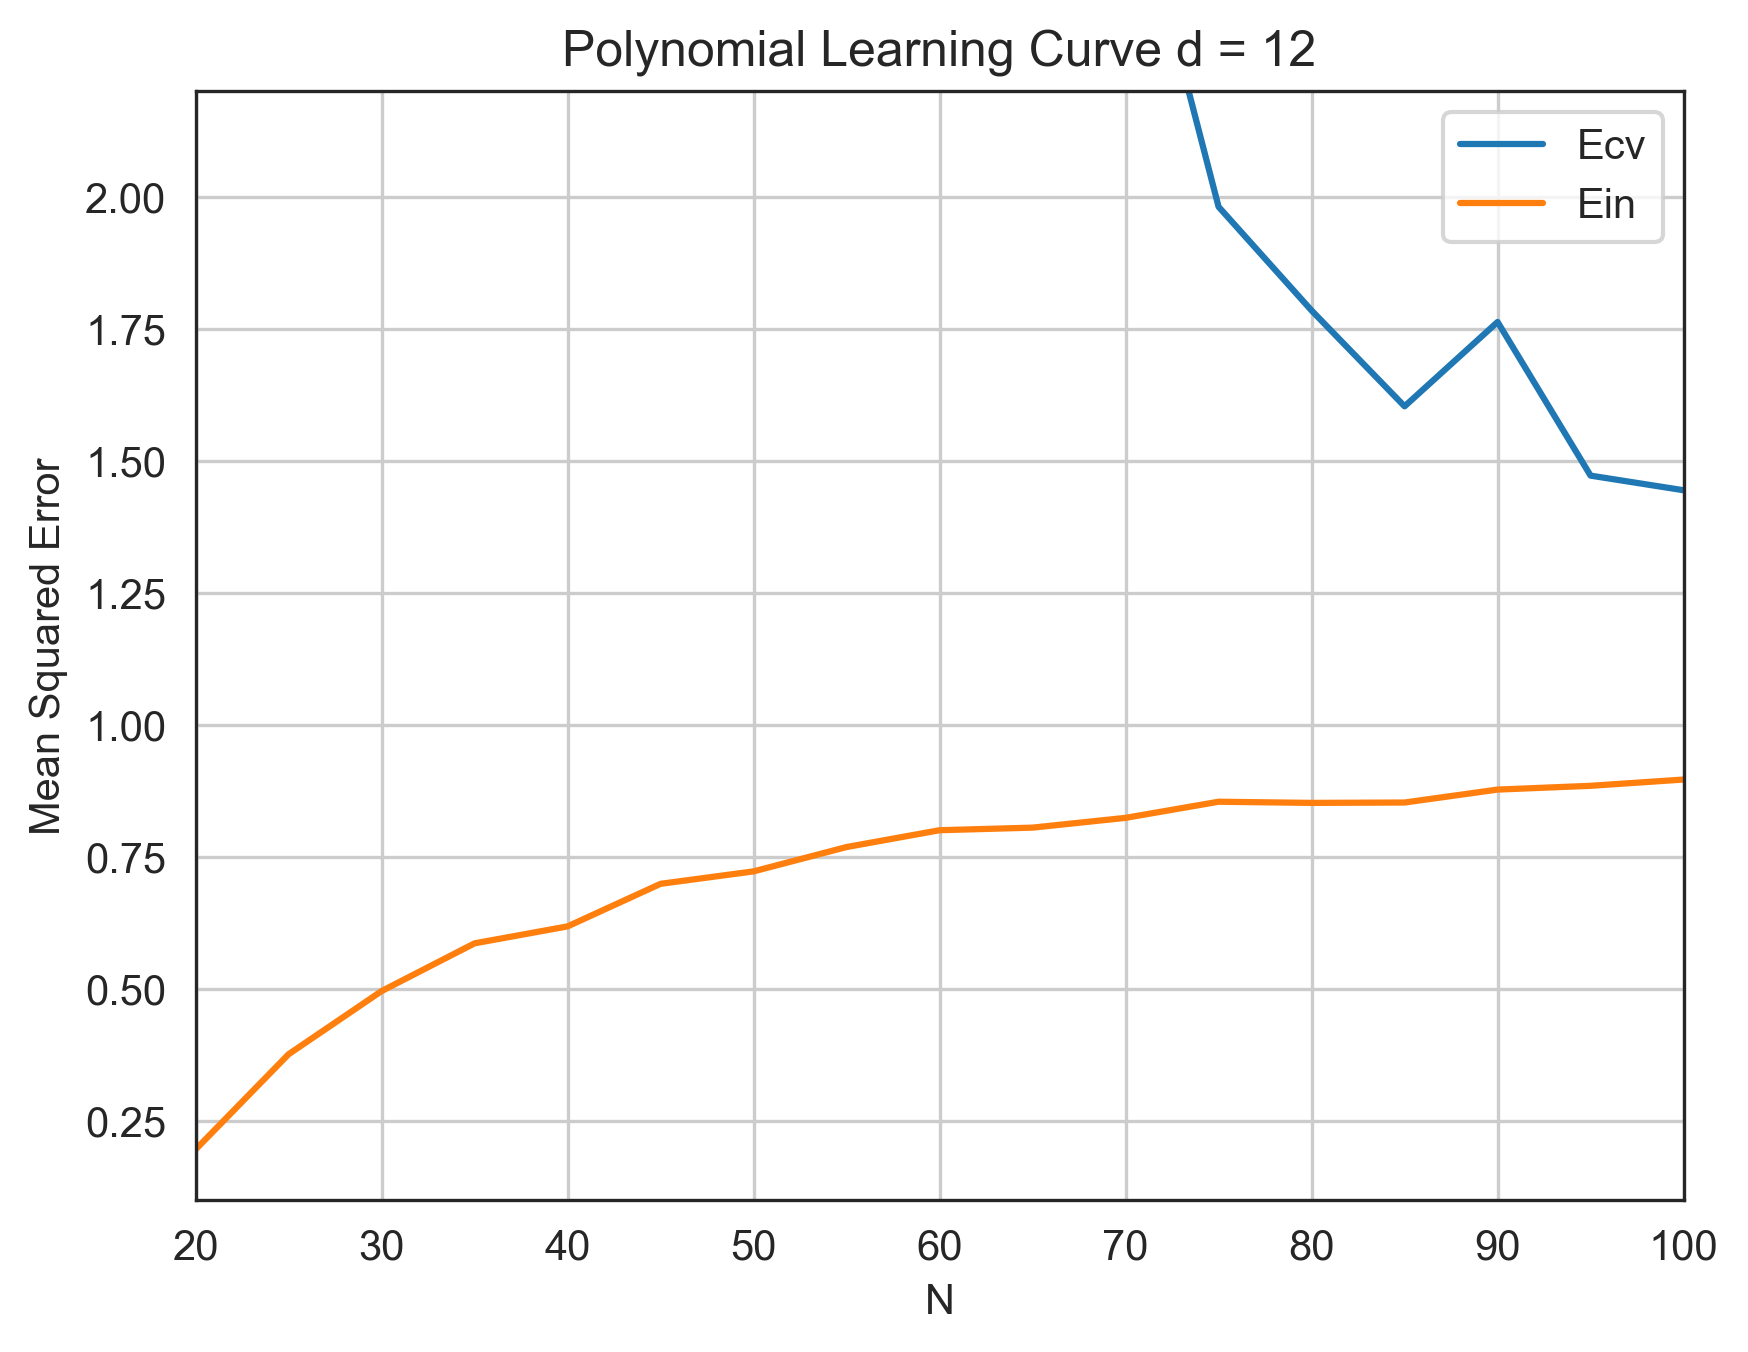
\includegraphics[scale=0.5]{figures/learncurve12.png}}
\caption{Learning Curves for Polynomial Model}\label{fig1}
\end{figure}

\item $d = 1$ has the highest bias. The value in which our learning curves asymptotically approaches as $N \to \infty$ is the bias, which is greatest for $d = 1$.
\item $d = 12$ has the highest variance. The distance between the bias and the out-of-sample error $\Eout$ is the variance.
\item The learning curve seems to show that the model wouldn't improve with additional points.
\item Training error is lower than validation error because the training error is the quantity which our learning algorithm is trying to minimize.
\item The $d = 6$ would perform best. It has a low bias and the discreptancy between the out-of-sample and in-sample performance shows that the parameter estimation is fairly consistent across samples.
\end{enumerate}
\item
\begin{enumerate}[label = \Alph*.]
\item The output file for the test is under the file name `simpleperceptron.html'.
\item In 2D, we see in Figure \ref{2d} that the perceptron shatters 3 points but not 4. Algebraically, we have $N + 1$ points in $N$-dimensions
\[ S = \{(\x_1, y_1), (\x_2, y_2), \ldots, (\x_{N+1}, y_{N+1})\} \]
such that for any $y_i$ where $i = 1, 2, \ldots N + 1$ that we choose, we must find a $\mathbf w$ and $b$ such that
\[ \mathbf w \cdot \x_i + b = y_i \qquad i = 1, 2, \ldots N+1. \]
We have $N$ unknowns in $\mathbf w$ and one unknown in $b$, which leads to $N + 1$ unknowns. This gives us the matrix
\[ \tilde X \tilde w = Y \]
where
\[ \tilde X = \begin{pmatrix} x_{11} & x_{12} & \cdots & x_{1N} & 1 \\ x_{21} & x_{22} & \cdots & x_{2N} & 1 \\ \vdots & \vdots & \ddots & \vdots & \vdots \\ x_{N+1, 1} & x_{N + 1, 2} & \cdots & x_{N + 1, N} & 1 \end{pmatrix}, \qquad \tilde w = \begin{pmatrix} w_1 \\ w_2 \\ \vdots \\ b \end{pmatrix}, \qquad Y = \begin{pmatrix} y_1 \\ y_2 \\ \vdots \\ y_{N +1} \end{pmatrix}. \]
If we can find non-trivial solutions to this equation, then we can shatter the data points since we can choose whatever labelling for the $y_i$'s. However, we know that $\tilde X$ is invertible, because if we set $Y = 0$, then this would imply that all $N + 1$ points are on the same hyperplane, implying that $\tilde w = 0$. This implies that $\tilde X$ is invertible, meaning that we have a unique solution $\tilde w$ for every choice of $Y$.

For $N + 2$ points, this may not be the case. If we add an extra row $\x_{N + 2}, 1$ to $\tilde X$, then we are not guaranteed that $\tilde X$ is invertible because $\tilde Y = 0$ does not imply $\tilde w = 0$. Therefore, $N + 1$ points are always separable in $N$-dimensions, but not $N + 2$ points.
\begin{figure}[h!]
\centering
\begin{tikzpicture}[scale = 0.87]
\draw [blue, fill] (0, 0) circle [radius = 0.07];
\draw [blue, fill] (3, 0) circle [radius = 0.07];
\draw [red, fill] (1.5, 2) circle [radius = 0.07];
\draw [dashed] (-1, 1) -- (4, 1);
\begin{scope}[shift={(5, 0)}]
\draw [blue, fill] (0, 0) circle [radius = 0.07];
\draw [red, fill] (3, 0) circle [radius = 0.07];
\draw [blue, fill] (1.5, 2) circle [radius = 0.07];
\draw [dashed] (0.75, -1) -- (3.85, 3);
\end{scope}
\begin{scope}[shift={(10, 0)}]
\draw [red, fill] (0, 0) circle [radius = 0.07];
\draw [blue, fill] (3, 0) circle [radius = 0.07];
\draw [blue, fill] (1.5, 2) circle [radius = 0.07];
\draw [dashed] (2.25, -1) -- (-0.85, 3);
\end{scope}
\begin{scope}[shift={(15, 0)}]
\draw [blue, fill] (0, 0) circle [radius = 0.07];
\draw [red, fill] (2, 0) circle [radius = 0.07];
\draw [blue, fill] (2, 2) circle [radius = 0.07];
\draw [red, fill] (0, 2) circle [radius = 0.07];
\end{scope}
\draw (-1, -1) -- (18, -1) -- (18, 3) -- (-1, 3) -- cycle;
\draw (4, -1) -- (4, 3);
\draw (9, -1) -- (9, 3);
\draw (14, -1) -- (14, 3);
\end{tikzpicture}
\caption{In two-dimensions, we see that in the case of three points, the data is always separable. However, the data can be non-separable in the case of four points.} \label{2d}
\end{figure}
\item The visualization is under the .html file ``perceptronns.html''. The algorithm never converges because there will always be one misclassified point. The PLA algorithm takes a misclassified point and modify the hyperplane until the misclassified point is correctly classified, but because there has to be at least one misclassified point, the PLA algorithm will never converge.
\end{enumerate}
\item
\begin{enumerate}[label = \Alph*.]
\item Just add a $x_0 = 1$ term. This way, $w_0 = b$ so that we can ignore the bias term and write
\[ f(\x) = \w^T \x. \]
\item We have
\[ \nabla_\w L(f) = - 2 \sum_{i = 1}^N (y_i - \w^T \x_i) \x_i \]
For SGD, we discard the summation and evaluate at a single point.
\[ \nabla_\w^{\text{SGD}} L(f(\x_i, y_i)) = -2 (y_i - \w^T \x_i) \x_i. \]
\item The plots are stored as gifs in the ``animation$n$.gif'' files.
\item In the first dataset, the SGD converges fairly evenly for the different $w_0$ points. In the second dataset, the SGD converges quicker for the $w_0$ points that are closer to the origin, i.e. $||w_0||$ implies faster convergence. This is simply due to the nature of the loss function for each dataset. In the first dataset, the further points had a steeper gradient so the different $w_0$ points had similar convergences while in the second dataset the closer points had a steeper gradient so the convergences differed.
\item The plot is shown in Figure \ref{etalearning}. We see that if we make $\eta$ too large ($\eta = 1$), then the $w$-updates are too large and never converge to the minimum-loss value, but instead just jumps around it, as shown in animation6.gif. When $\eta$ becomes too large ($\eta = 10$), $w$ actually diverges because the gradient of the loss function becomes very large. When there are multiple optimas, different $w_0$'s can converge to different $w_N$'s. So it is important to have a large enough $\eta$ where we can randomly jump out of an optima, but small enough where it will converge.
\begin{figure}[h!]
\centering
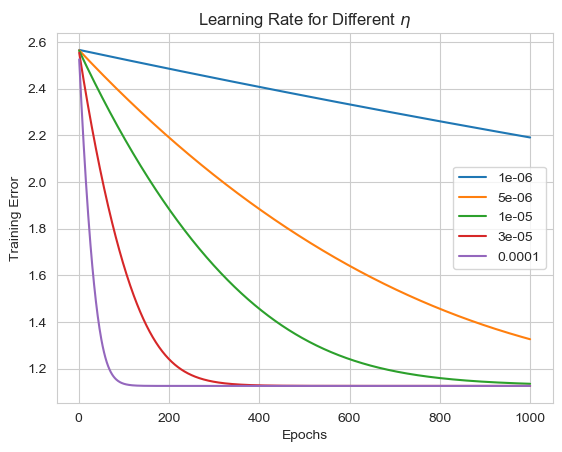
\includegraphics[scale=0.75]{epochlearning.png}
\caption{Learning Curve for Differing $\eta$.} \label{etalearning}
\end{figure}
\item For the larger dataset from the sgd\text{\textunderscore}data.csv file with $\eta = e^{-15}$, we get
\[ w = [-0.22788371, -5.97853503, 3.98839083, -11.85700488, 8.91129436] \] 
\item We get a learning curve as shown. We can see that the larger $\eta$ results in faster convergence up to a certain limit. When the curves flatten out, this means that the weights have converged and any SGD update to the weights will just oscillate around the optimal value.
\begin{figure}[h!]
\centering
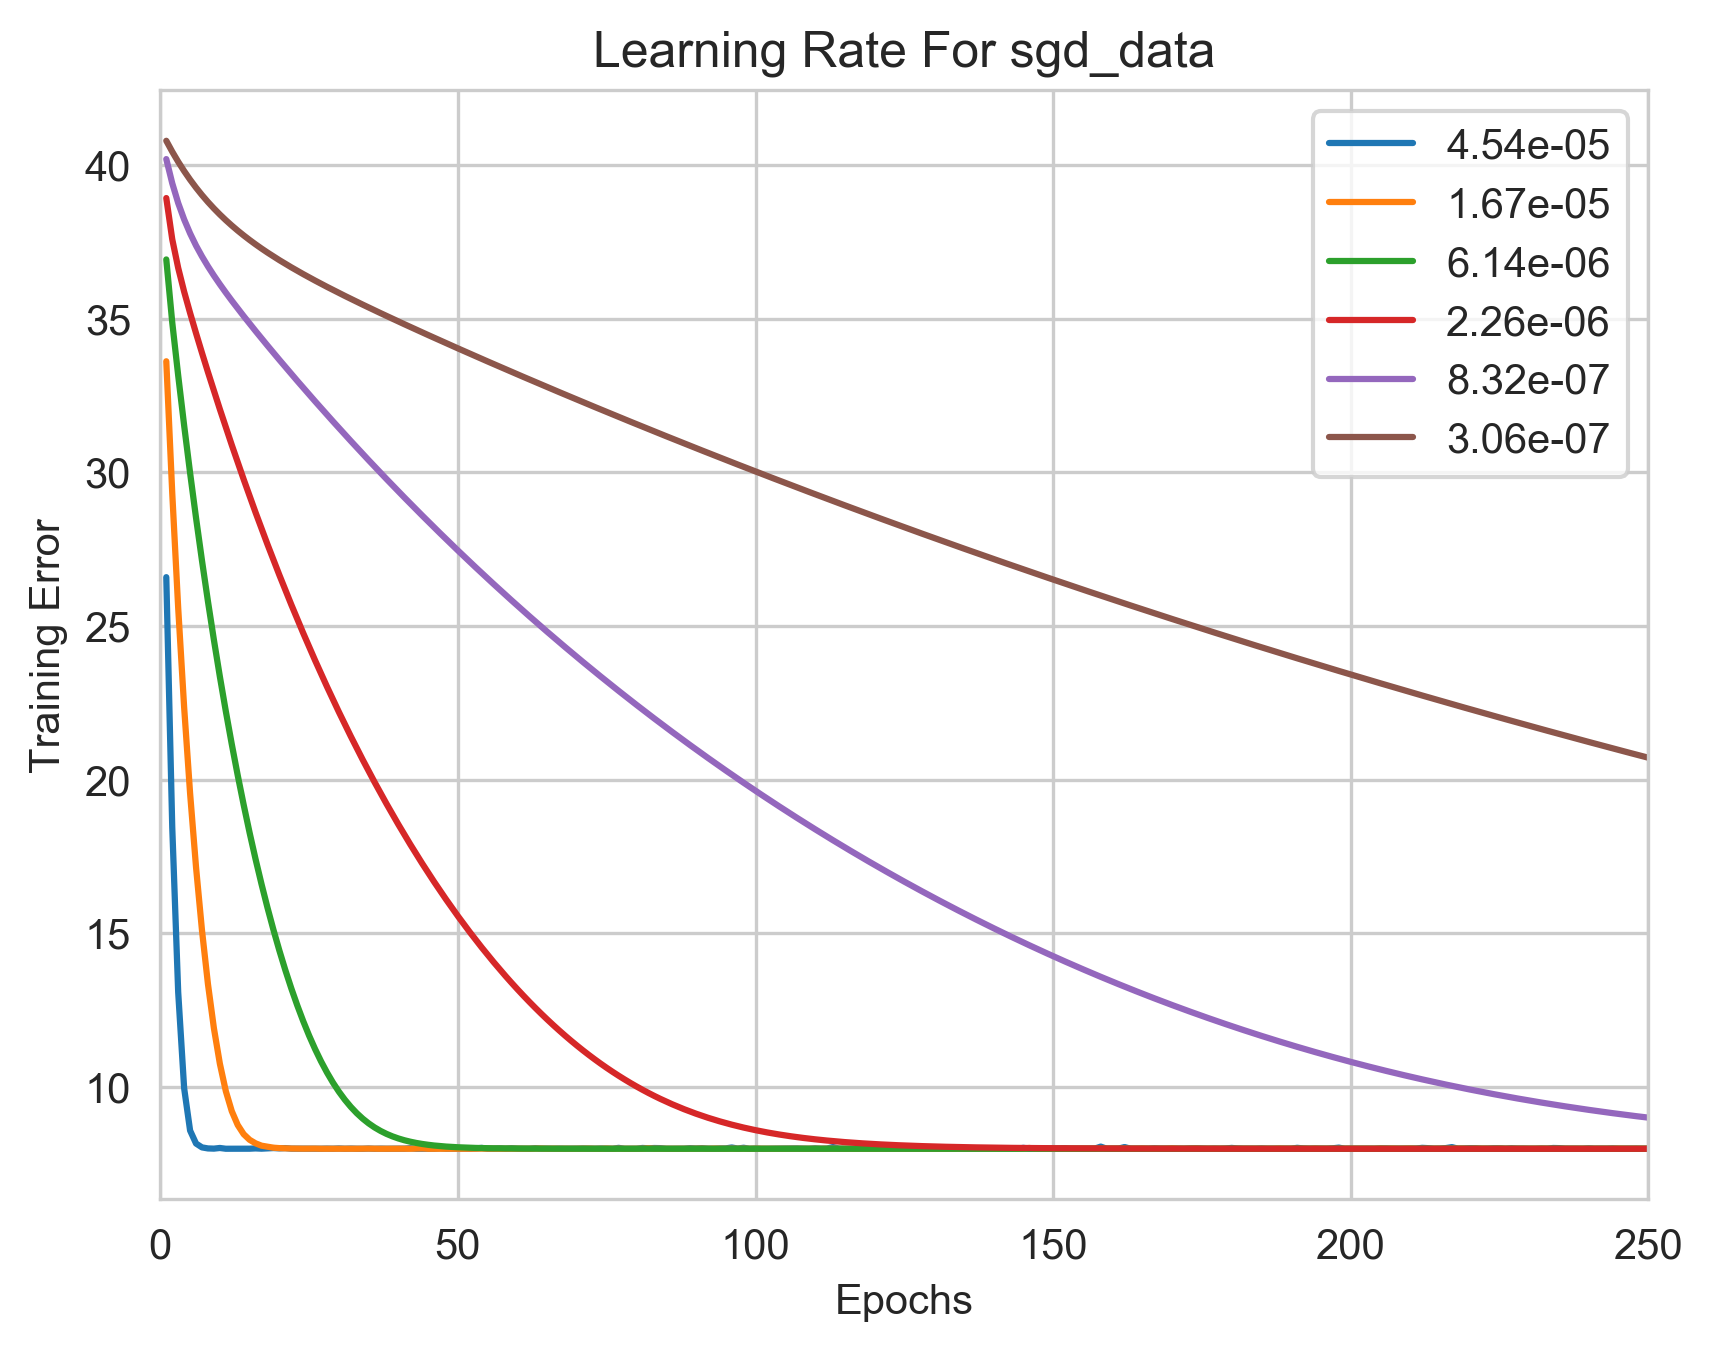
\includegraphics[scale=0.75]{epochlearning2.png}
\caption{Learning Curves for Larger Dataset} \label{etalearning2}
\end{figure}
\item The SGD value is
\[ w_{\text{SGD}} = [-0.31646018, -5.97846778, 4.0156245, -11.94060225, 8.98594131] \]
and the analytical value is
\[ w_{\text{analytical}} = [-0.31644251, -5.99157048, 4.01509955, -11.93325972, 8.99061096]. \]
This is less than a 0.1 percent difference. More explicitly,
\[ \frac{||w_{\text{SGD}} - w_{\text{analytical}}||}{||w_{\text{analytical}}||} < 0.001. \]
\item Yes, when the data is very large and we have online learning where the data keeps updating, we don't want to re-train the entire data set (matrix multiplication has awful computational times for large matrices). SGD is much more computationally friendly.
\item We can use
\[ |L(w_i) - L(w_{i + 1}| < \epsilon \]
where $\epsilon$ is some precision we use. We could also use
\[ ||w_i - w_{i + 1}|| < \epsilon. \]
The latter is probably better because two separate weights could have similar losses.
\item The SGD algorithm will converge such that the weight vector converges to a specific value. The perceptron may not converge if the data is not separable. Thus, we would have to decide when to stop the PLA algorithm if it's not separable manually, whether that is checking for the lowest error.
\end{enumerate}
\end{enumerate}


\end{document}